\documentclass[french]{beamer}

\usepackage[utf8]{inputenc}
\usepackage[T1]{fontenc}
\usepackage{lmodern}
\usepackage{amsmath, amssymb}

\usepackage{babel}


%CHOIX DU THEME et/ou DE SA COULEUR
% => essayer différents thèmes (en décommantant une des trois lignes suivantes)
\usetheme{PaloAlto}
%\usetheme{Madrid}
%\usetheme{Copenhagen}

% => il est possible, pour un thème donné, de modifier seulement la couleur
%\usecolortheme{crane}
%\usecolortheme{seahorse}

%\useoutertheme[left]{sidebar}


%Pour le TITLEPAGE
\title{Projet de Recherche}
\author[]{TOULLALAN Antoine MENDAS Rosa}
\date{Lundi 15 Février (6e réunion)}


\begin{document}

\begin{frame}
	\titlepage
\end{frame}
\section{Résumé de l'article}
\begin{frame}{Qu'est ce que ASCENT?}
L’article présente ASCENT, un outil qui s’ajoute aux DHT qui contienne potentiellement des noeuds mal intentionnés. \\ASCENT fournit un certificat attestant qu’une transaction a bien été effectuée entre un client et un service dans un temps donné.\\ On a ainsi une garantie que les données certifiées contenues dans le DHT ne sont pas corrompues.\\
\end{frame}
\begin{frame}{Description du système}
ASCENT est mis en place dans un certain système comportant les éléments suivants :\\Le premier élément de base est évidemment un \textbf{DHT} composée de noeuds. Chaque noeud est associé à une clé privée et une clé publique qui servent à les identifier notamment lors des transactions.\\Le deuxième élément est un \textbf{système de réputation} qui identifie les noeuds "honnêtes" et les noeuds mal intentionnés (on utilisera le système WTR), ce système est associé à une fonction R(X)=Y ou X est un noeud et Y la probabilité que X soit un  noeud de confiance.
\end{frame}
\begin{frame}{Description du système}
Le troisième élément est un \textbf{ensemble de noeuds de confiance}, qui permet à chaque noeud de confiance d'avoir une table contenant une partie des autres noeuds de confiance (pour cela on utilisera l'algotithme CORPS)->l'ensemble des noeuds de confiance sont organisés dans un anneau de confiance ainsi chaque noeud de confiance K est associé avec un noeud Kroot qui se situe dans l'anneau de confiance.
\end{frame}
\begin{frame}{Fonctionnement de ASCENT}
Si un noeud n'a pas de table de noeuds de confiance , on prend un noeud K et on demande à Kroot sa table d'anneaux de confiance, on regarde si cette table est bien valide (elle contient bien des noeuds de confiance) si la table n'est pas valide le noeud construit sa table de noeuds valide de zero.\\
\end{frame}
\begin{frame}{Fonctionnement de ASCENT}
Soit un service associé à un noeud , pour utiliser ce service càd effectuer une transaction avec ce noeud, le noeud A va d'abord envoyer un message  "RequestInit" à l'ensemble des noeuds de confiance S de Sroot,(Sroot étant le noeuds le plus susceptible d'être associé au service ). Si au moins la moitié des noeuds de S répondent favorablement, La transaction a lieu.\\
Lors de la transaction le noeud A signe chaque message avec sa clé privée et au moins la majorité des noeuds de S doit lui donner la même réponse sinon la transaction prend fin.
\end{frame}
\begin{frame}{Fonctionnement de ASCENT}
Après le "RequestInit" de A, les noeuds de S vont chercher à obtenir la  certification de A qui se situe dans un autre ensemble C de noeuds. Lorsqu'un noeud de C recoit les notifications d'au moins la moitié des noeuds de S concernant la transaction, alors le noeud de C émet le certificat. Lorsque les certificats sont reçus, les noeuds S répondent favorablement et la transaction a lieu.\\
Il y a des algorithmes permettant de ne pas perdre de certificats de noeuds lors de départs de noeuds.
\end{frame}
\begin{frame}
  \frametitle{Réseaux de Petri Symétriques}
  
  \begin{itemize}
      \item Stocker les configurations d’un système sans tenir compte des symétries\\
      \item Système complet trop complexe pour être formellement modélisé
      \item On s'intéresse à une seule transaction et donc à un acteur et son leafset: celui offrant le service, et celui traitant de la certification
    \end{itemize}
On émet pour hypothèses que:\\ 
L’algorithme DHT nous fournit un nombre constant de nœuds dans le leafset\\
Chaque acteur attend un nombre n de réponses au lieu des |L|/2 + 1 habituelles\\
Le service est basé sur une communication bidirectionnelle\\
\end{frame}

\begin{frame}
  \frametitle{Modèle formel}
  
  \begin{center}
  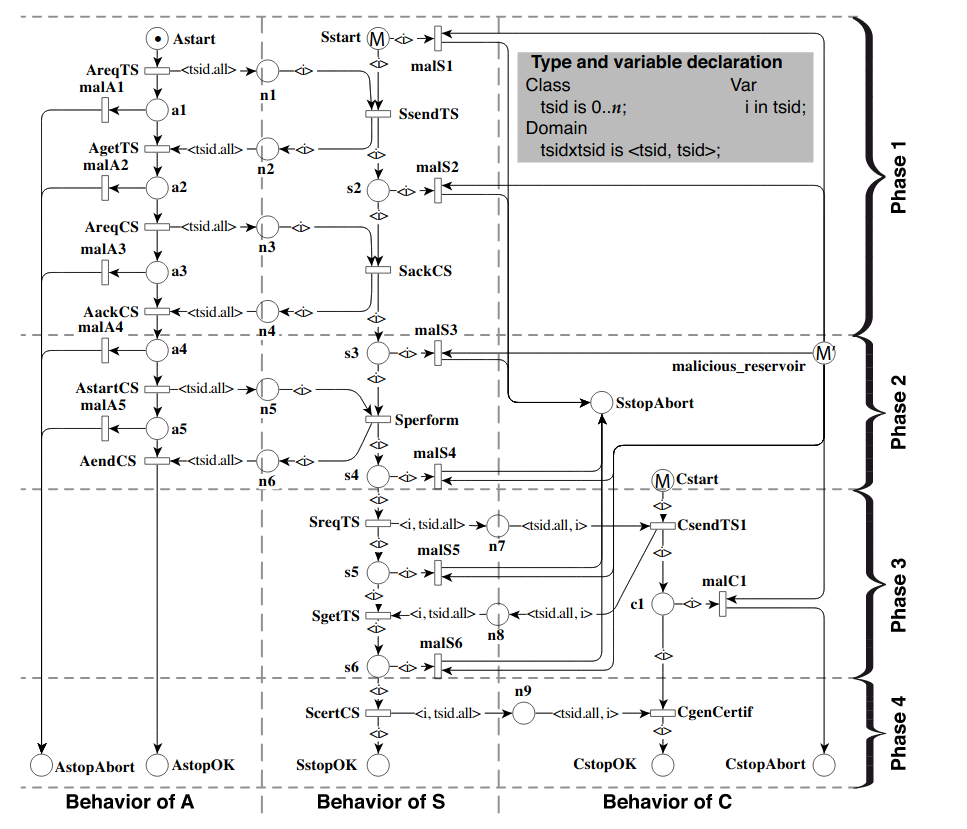
\includegraphics[scale=0.25]{PR1.png}
  \end{center}
\end{frame}
\section{Extension du Leaf Set}
\begin{frame}{extension du LeafSet}
\begin{center}
\includegraphics[scale=0.28]{"schema_extension_leafset"}
\end{center}
\end{frame}
\begin{frame}{extension du LeafSet: Petri}
\begin{figure}
\includegraphics[width=0.7\linewidth]{"petri_leafset"} 
\end{figure}
\end{frame}
\begin{frame}
\begin{Large}
p1: Li est vide, C non choisit\\

p2: C=	$ L_{-|L|/2} $ \\

p3: C=	$ L_{+|L|/2} $ \\

p4: L' est le Leafset de C	\\

p5: On assigne $ L'_{j} $ à Li, Li non vide\\


t1: On a -|L|/2<i<0\\
t2: On a 0<i<+|L|/2\\
t3: C transmet son Leaf Set\\
t4: On choisit la case $ L'_{j} $ de L' qui correspond le mieux à Li\\
\end{Large}
\end{frame}
\begin{frame}{extension du LeafSet: Petri coloré}
\includegraphics[width=0.58\linewidth]{"petri_colore_leafset"} 
\end{frame}
\begin{frame}
  \frametitle{Présentation de la modélisation}
  \begin{center}
  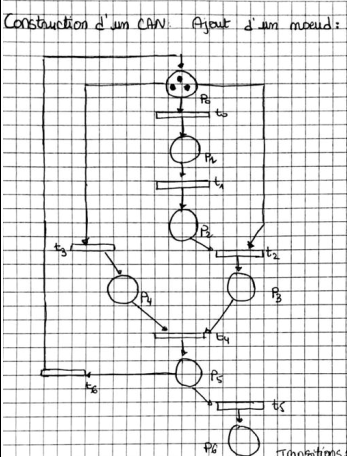
\includegraphics[scale=0.45]{PR2.png}
  \end{center}
\end{frame}
  
 \begin{frame}
  \frametitle{Présentation de la modélisation}
  P0: Noeud à inserer\\
  P1: Noeud Bootstrap\\
  P2: Liste des noeuds actifs\\
  P3: Noeud aléatoire\\
  P4: Point aléatoire\\
  P5: Noeud responsable de la zone contenant P\\
  P6: Noeud dans CAN\\
  ------------ \\
  T0: Trouver frâce à DNS IP du Bootstrap c\\
  T1: c établi une liste des noeuds actifs du CAN\\
  T2: Noeud choisi aléatoirement pour le routage\\
  T3: Noeud à inserer choisi aléatoirement point P\\
  T4: Router un message JOIN vers le noeud x responsable de la zone contenant P\\
  T5: x divise sa zone et accorde la moitié\\
  T6: x refuse de diviser sa zone

 
\end{frame}

\begin{frame}
  \frametitle{Sources}
  
  \begin{itemize}
    \item  https://hal.sorbonne-universite.fr/hal-01547514/document
    
    \item https://pages.lip6.fr/Olivier.Marin/Publis/corps-CJ2011.pdf

    \end{itemize}
  
\end{frame}


\end{document}
\end{document}